\section{Scaling Performances}


\begin{figure*}%[ht]
%  \vskip -0.5cm 
  \begin{center}
    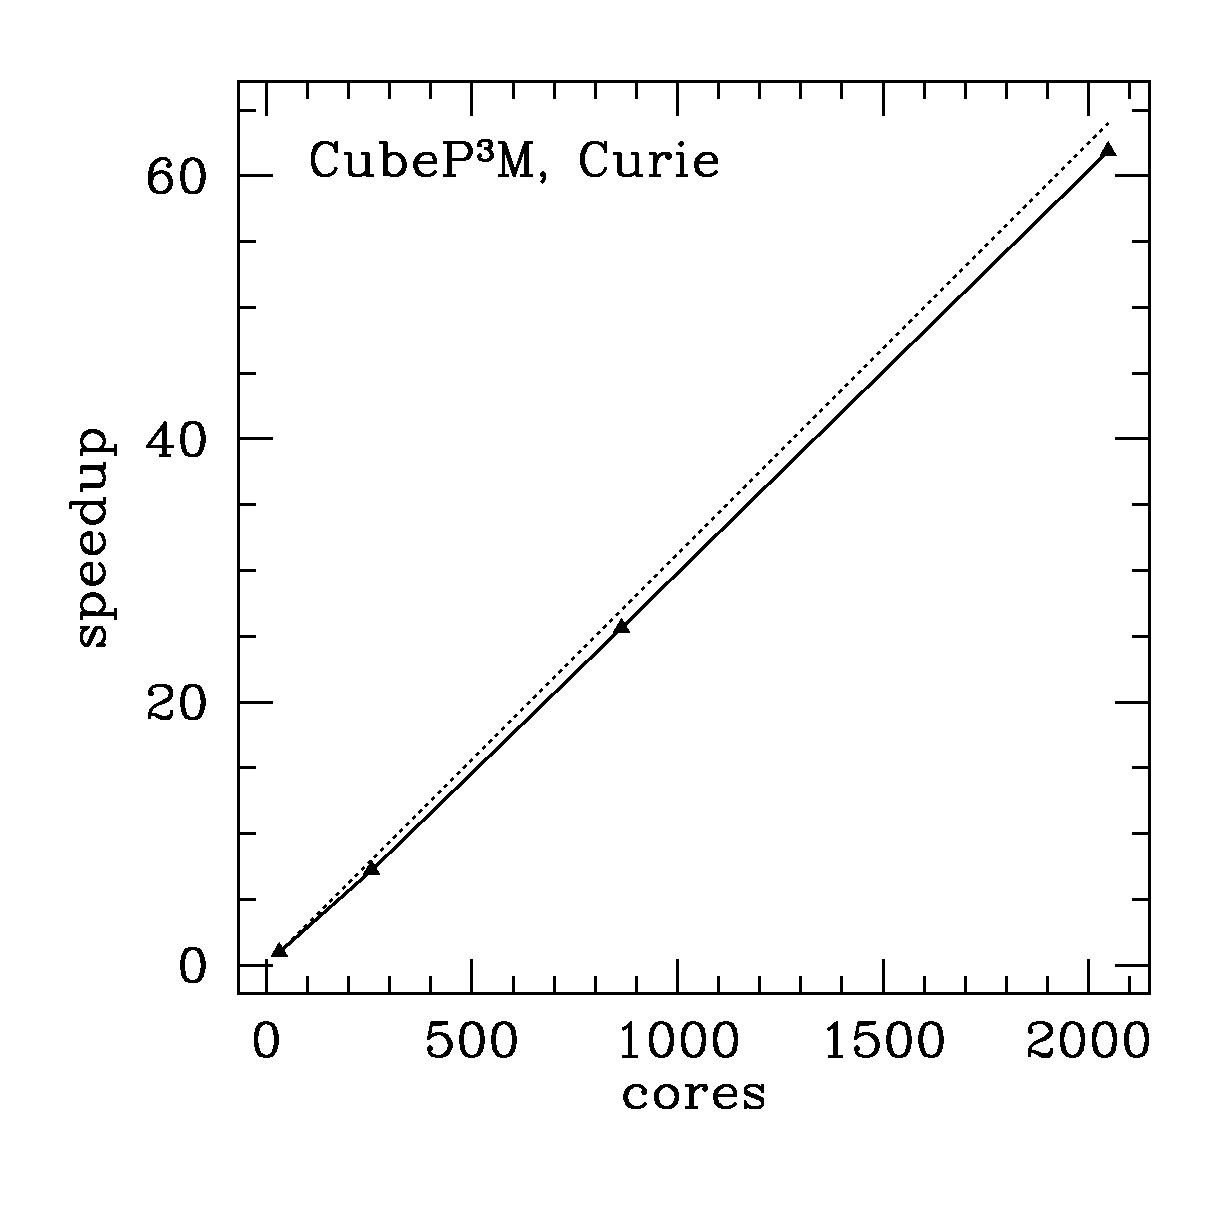
\includegraphics[width=3.2in]{graphs/scaling_cubep3m_curie.eps}
    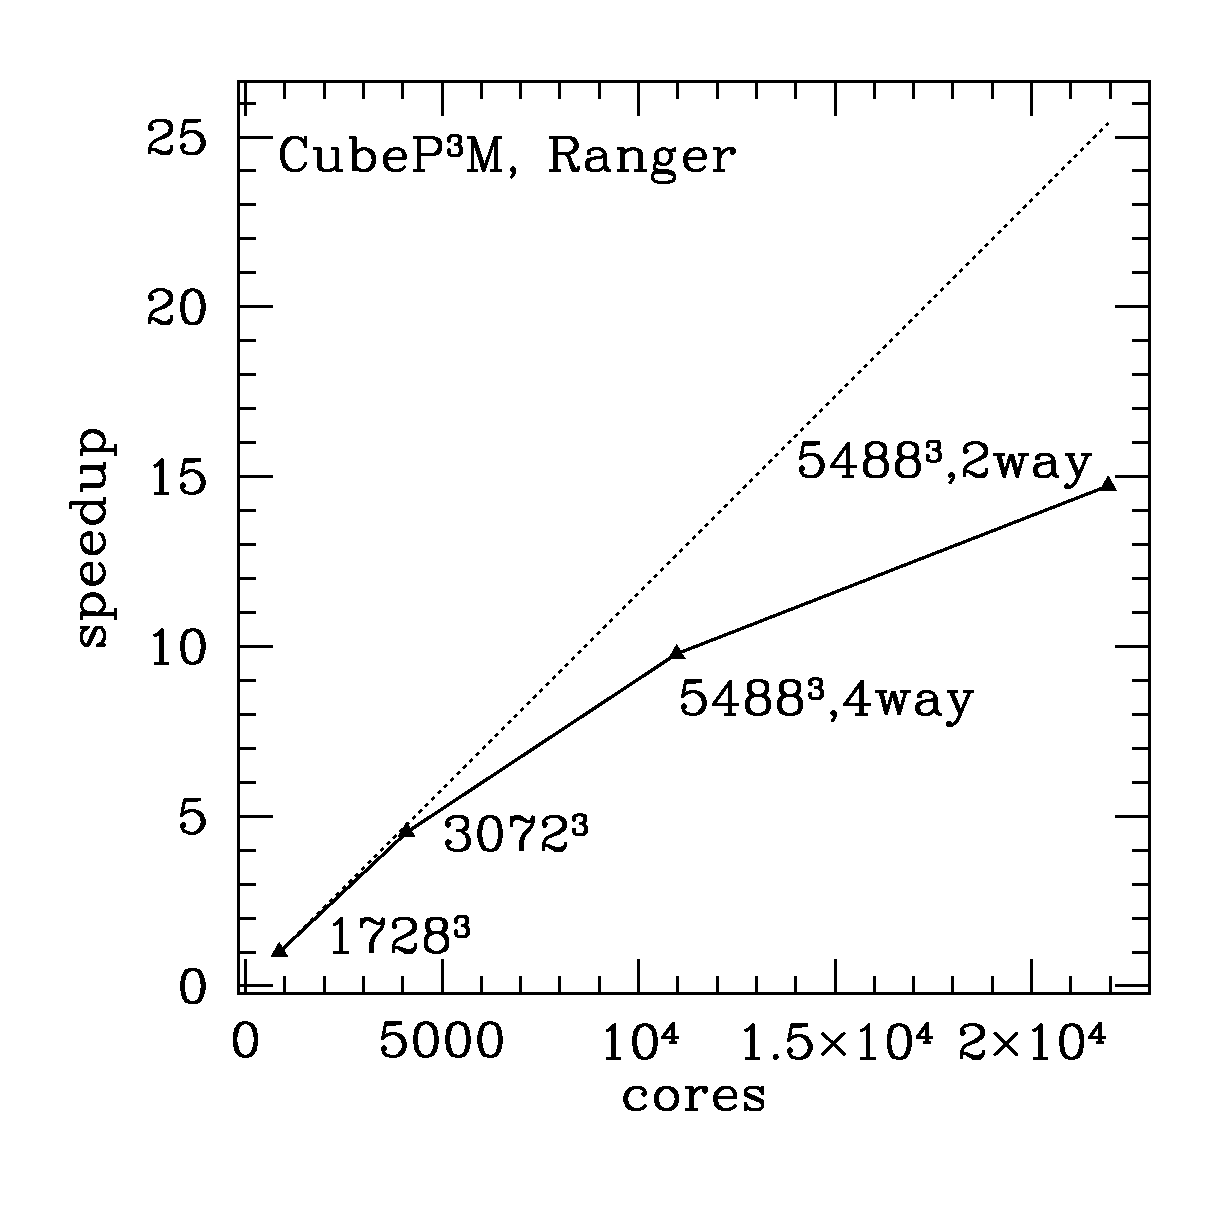
\includegraphics[width=3.2in]{graphs/scaling_cubep3m_new.eps}
%  \vskip -1.2cm 
%  \vskip -0.5cm 
  \caption{Scaling of {\small CUBEP3M} on Curie fat nodes (left) and 
    on Ranger TACC facility for very large number of cores (right). Plotted is the code speedup 
    ($N_{\rm particles}^3/t_{\rm wallclock}$) against core count, normalized by the smallest run 
    in each case. Dashed line indicates the ideal weak 
    scaling. The data is listed in Table \ref{summary_scaling_table}.
    \label{scaling}
% \vskip -0.9cm 
}
\end{center}
\end{figure*}

\begin{table*}%[ht]
  \vskip -0.5cm 
  \begin{center}
\caption{Scaling of {\small CUBEP3M} on Curie. Speedup is 
scaled to the smallest run.}
\label{summary_scaling_table}
\begin{tabular}{@{}|llllll|}
\hline
number of cores & speedup & ideal speedup & absolute timing (min) & 
$N_{\rm particles}$& box size ($h^{-1}$Mpc)
\\[2mm]\hline
%\hline
32  &  1.00 & - &3.2 & $256^3$ & 256\\
256  & 7.21 & 8 &3.55 & $512^3$  & 512\\
864  & 25.63 & 27 &4.8 & $864^3$  & 864\\
2048  & 61.87 & 64 &26.48 & $2048^3$ & 2048 \\
\hline
\end{tabular}
\caption{Scaling of  {\small CUBEP3M} for large number of cores 
(on Ranger). Speedup is scaled to the smallest run.}
\label{summary_scaling_table2}
\begin{tabular}{@{}|llllll|}
\hline
number of cores & speedup & ideal speedup & absolute timing (min) & 
$N_{\rm particles}$& box size ($h^{-1}$Mpc)
\\[2mm]\hline
%\hline
864    & 1.00  & -    &258   & $1728^3$  & 6.3\\
4096   & 4.53  & 4.74 &320   & $3072^3$  & 11.4\\
10976  & 9.78  & 12.7 &845   & $5488^3$  & 20\\
21952  & 14.73 & 25.4 &561   & $5488^3$  & 20 \\
\hline
\end{tabular}
\end{center}
  \vskip -0.7cm 
\end{table*}

%the Ranger system at the Texas Supercomputing
%Center (in top 20 in the world) which is a SunBlade x6420 
%with AMD x86\_64 Opteron Quad Core 2300 MHz (9.2 GFlops)
% ``Barcelona'' processors and Infiniband networking. It has 
%a total of 62976 computing cores and 125952 GB of total 
%memory. Its nodes consist of 4 Quad Core processors and 32 GB 
%of shared RAM. For efficiency reasons (local memory access) we 
%typically use smaller MPI 'nodes' consisting of one Quad Core 
%processor and 8 GB of RAM. 

The parallel algorithm of {\small CUBEP$^3$M} is designed for ``weak'' 
scaling, i.e. if the number of cores and the problem size 
increase in proportion to each other, then for ideal scaling the 
wall-clock time should remain the same, in contrast to ``strong'' 
scaling, whereby the same problem solved on more cores should take 
proportionately less wall-clock time. This weak scaling requirement 
is dictated by the problems we are typically aiming towards (very 
large and computationally-intensive) and our goals, which are to 
address such large problems in the most efficient way, rather than 
for the least wall-clock time. Furthermore, there is no explicit 
load balancing, thus the code is most efficient if the sub-domains
contain roughly equal number of particles, which is true for most
cosmological-size volumes, but not for e.g. simulations of a single
highly-resolved galaxy. 

%Since the current Curie is using Intel Nehalem architecture, while 
%the thin Curie nodes will use the newer Westermere Intel architecture, 
%we also show the scaling of our code on the Westermere-based Lonestar 
%computer at the Texas Advanced Computing Centre 
 
The scaling was tested with a dedicated series 
of simulations with increasing size and number of cores on the `fat'' 
(i.e. large-memory) nodes of the supercomputers Curie at TGCC in France. 
Our results are shown in Fig. \ref{scaling} and in 
Table \ref{summary_scaling_table}. For appropriate direct comparison,
all simulations were performed using the same particle mass 
($M_{\rm particle}=1.07\times10^{11}M_\odot$) and force resolution 
(softening length 50 $h^{-1}$kpc). The box sizes used range from 256 $h^{-1}$Mpc
to 2048 $h^{-1}$Mpc, and the number of particles from $256^3$ to $2048^3$.
Simulations were run on 32 up to 2048 computing cores starting from 
redshift $z=100$, and evolving until $z=0$. Our results show excellent scaling, within 
$\sim3\%$ of the ideal one, for up to 2048 cores. 

We have also ran {\small CUBEP$^3$M} on a much larger number of cores, 
from 8000 to up to 21,976, with $5488^3$-$6000^3$ (165 to 216 billion) 
particles on Ranger at the Texas Advanced Computing Centre (SunBlade 
x6420 with AMD x86\_64 Opteron Quad Core 2300 MHz (9.2 GFlops)
``Barcelona'' processors and Infiniband networking, a total of 62,976 
computing cores and 125,952 GB of total memory. Its shared-memory nodes 
consist of 4 Quad Core processors and 32 GB of RAM.) and JUROPA 
at J\"ulich Supercomputing Centre in Germany (Intel Xeon X5570 
(Nehalem-EP) quad-core, 2.93 GHz, Infiniband networking, a total of 17,664
computing cores and 52 TB of total memory. Its shared-memory nodes 
consist of 2 Quad Core processors and 24 GB of RAM). Since it is not 
practical to perform dedicated scaling tests on such large number 
computing cores, we instead use data extracted from production runs, 
as listed in Table \ref{summary_scaling_table2}. We have found the 
code to scale quite well, within 1.5\% of ideal up to 4,096 cores. 
For very large number of cores (10,976) the scaling is slightly worse,
but still within $\sim20\%$ of ideal, due to increased communication 
costs, I/O overheads (a single timeslice of $5488^3$ particles is 3.6 TB)
and load balancing issues. These first three Ranger runs were performed 
with 4 MPI processes and 4 threads per Ranger node ('4way') (using the 
specially-provided {\it tacc\_affinity} NUMA script to bind the memory 
usage to local core, thus ensuring memory affinity. This is important 
because the 32 GB RAM/node on Ranger (and other computers with 
multi-processor sockets) are actually not equal-access and the local 
8 GB memory of each processor has much shorter access time).

Furthermore, due to the very strong clustering of structures at those small 
scales, some of the cuboid sub-domains came to contain well above the 
average number of particles, thereby requiring more memory per MPI process
in order to run. As a consequence, throughout most of the evolution the 
largest two of these simulations were run with 4096 and 21,952 cores and 
with only 2 MPI processes and 8 threads per Ranger node (2way), which on 
Ranger allows using up to 16 GB of RAM per MPI process. In order to insure 
local memory affinity a special NUMA control script (which we called {\it 
tacc\_affinity\_2way}) 
was developed for us by TACC staff and was used by us to run more efficiently 
in this mode. However, this not-fully-local memory access does affect the 
performance somewhat, as does the imperfect load balancing in such situations,
as seen by the rightmost point on the scaling plot. The scaling in this case
is 42\% below the ideal, although we note that we still get $\sim1.5$ speedup
from doubling the core count, even given these issues. Overall the
code scaling performance is thus quite satisfactory and it clearly 
scales very well to extremely large number of cores and can therefore 
do very large problems efficiently, utilizing the next generation 
Petascale systems. 

Finally, we note that several special fixes had to be developed by TACC 
and JUROPA staff in order for our largest runs to work properly and to be 
able to use the software libraries we required (MPICH and FFTW), as those 
latter exhibited serious problems when applied to runs of such 
unprecedented size. 

Real time versus size, bottle neck, description of the largest runs, etc.
{\bf (Hugh, do you have anything you would like to share 
concerning the largest runs you did on Blue Gene? )} 
